\section{常微分方程周期性}

\begin{figure}[H]
\centering
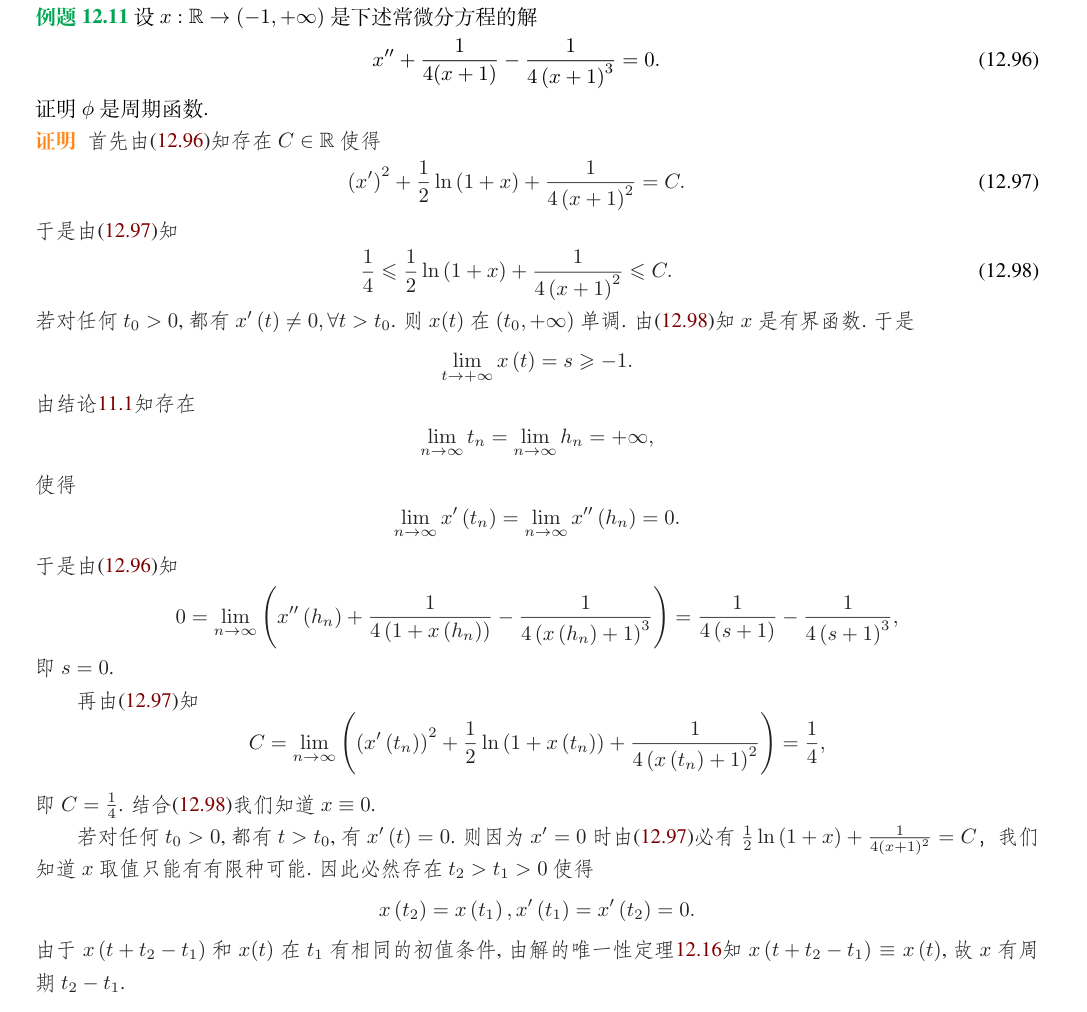
\includegraphics[width=\textwidth]{1-常微分方程周期性-2025051515.png}
% \caption{}
\label{}
\end{figure}

\begin{exercise}[yau-2020]
\begin{figure}[H]
\centering
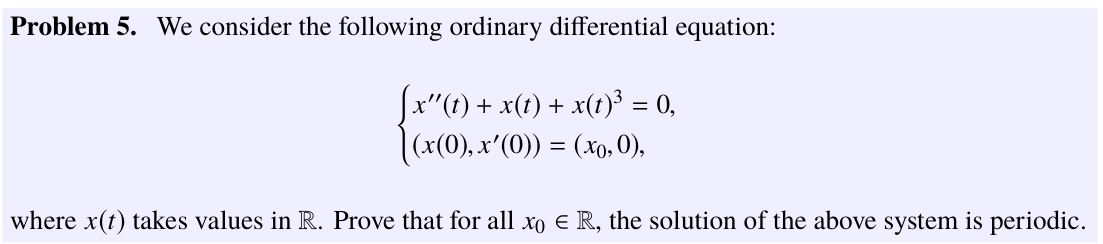
\includegraphics[width=\textwidth]{2-常微分方程周期性-2025051515.png}
% \caption{}
\label{}
\end{figure}
\end{exercise}
\begin{proof}
There exists constant $C$, s.t.
\[
(x')^2+x^2+\frac{1}{2}x^{4}=C
\]
Then $x$ is bounded since
\[
0\leq x^2+\frac{1}{2}x^{4}\leq C
\]
Then $\lvert x \rvert<M$ for some $M>0$.

If $\forall t_0>0$, we have $x'(t)\neq0,\forall t>t_0$, then $x(t)$ is monotonic.
\[
\lim_{ t \to +\infty } x(t)=s\in \mathbb{R}
\]
Thus there exists $\{ t_n \}\to \infty,\{ h_n \}\to \infty$, s.t.
\[
\lim_{ n \to \infty } x'(t_n)=\lim_{ n \to \infty } x''(h_n)=0
\]
Then
\[
\lim_{ n \to \infty } (x'(t_n))^2+x^2(t_n)+x^{4}(t_n)=C\Rightarrow s^2+\frac{1}{2}s ^{4}=C
\]
\[
\lim_{ n \to \infty } x''(h_n)+x(h_n)+x^{3}(h_n)=0\Rightarrow s+s ^{3}=0
\]
Therefore $s=0$; $C=0$; thus $x\equiv0$.

If $\forall t_0>0$, there exists $t>t_0$, s.t. $x'(t)=0$. There is a sequence $\{ t_n \}\to \infty$, s.t. $x'(t_n)=0$. Then
\[
x^2(t_n)+x^{4}(t_n)=C
\]
which has only finite solutions; thus there exists (WLOG) $t_1,t_2$ s.t.
\[
x(t_1)=x(t_2)\qquad x'(t_1)=x'(t_2)=0
\]
Then $x(t-t_1+t_2)$ and $x(t)$ has the same initial condition at $t_1$. The solution is unique since
\[
x''=f(t,x,x')=-x-x^3
\]
Let $f(t,\boldsymbol{y})=-y_1-y_1^3$, then
\[
\begin{aligned}
\lvert f(t,\boldsymbol{y})-f(t,\boldsymbol{z}) \rvert & =\lvert -y_1-y_1^3+z_1+z_1^3 \rvert  \\
 & =\lvert y_1-z_1 \rvert \lvert 1+y_1^2+z_1^2+y_1z_1 \rvert   \\
 & \leq (1+3M^2)\lvert y_1-z_1 \rvert 
\end{aligned}
\]
$f$ is Lipschitz on $\boldsymbol{y}$, which guarantees the uniqueness. Hence $x$ is periodic with period $t_2-t_1$.
\end{proof}
